\subsubsection{Signal conditioner (Galileo E1 + E5a)}


\begin{table}[H]
  \centering
  \footnotesize
  \resizebox{\ifdim\width>\linewidth\linewidth\else\width\fi}{!}{%
  \begin{tabular}{l>{\centering\arraybackslash}p{4.2cm}>{\centering\arraybackslash}p{4.2cm}}
    \hline
    \textbf{Channel} & \textbf{ch0 (E1)} & \textbf{ch1 (E5a)} \\
    \hline
    File format & ci8 & ci8 \\
    Source item type & ibyte & ibyte \\
    Data type adapter & Ibyte\_To\_Complex & Ibyte\_To\_Complex \\
    Input filter & Pass\_Through & Pass\_Through \\
    Resampling & $\times$5 zero-order hold, offline (\texttt{upsample\_iq.py}) & Pass\_Through \\
    Rate [MS/s] & 4 $\to$ 20 & 20 $\to$ 20 \\
    \hline
  \end{tabular}}
  \caption{Signal conditioner: recorded format and rate to gnss-sdr's internal \texttt{gr\_complex} stream; both bands are read in lockstep by one \texttt{Multichannel\_File\_Signal\_Source}.}
\end{table}

\subsubsection{Acquisition (Galileo E1 + E5a)}
Two-dimensional search over code delay and Doppler (one channel per band dumped; the others behave alike).

\begin{figure}[H]
  \centering
  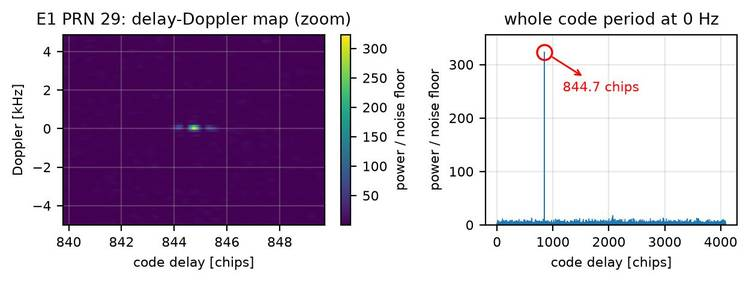
\includegraphics[width=1.0\linewidth]{gnss_sdr/x310_20261024T190000Z/galileo_acq_1B.jpg}
  \caption{Acquisition, E1: delay--Doppler search of PRN 29; one sharp peak (test statistic 450 vs threshold 52) at 0~Hz and 844.7~chips.}
\end{figure}

\begin{figure}[H]
  \centering
  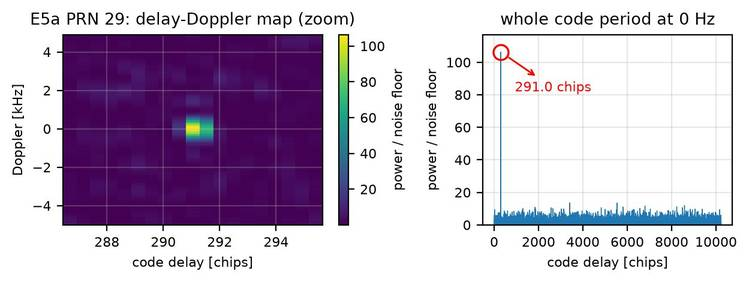
\includegraphics[width=1.0\linewidth]{gnss_sdr/x310_20261024T190000Z/galileo_acq_5X.jpg}
  \caption{Acquisition, E5a: delay--Doppler search of PRN 29; one sharp peak (test statistic 149 vs threshold 49) at 27~Hz and 291.0~chips.}
\end{figure}

\begin{table}[H]
  \centering
  \footnotesize
  \resizebox{\ifdim\width>\linewidth\linewidth\else\width\fi}{!}{%
  \begin{tabular}{lrrrr}
    \hline
    \textbf{Band} & \textbf{Attempts} & \textbf{Detections} & \textbf{Detected PRNs} & \textbf{Best statistic / threshold\footnotemark} \\
    \hline
    E1 & 4 & 1 & 29 & 8.7 \\
    E5a & 1 & 1 & 29 & 3.0 \\
    \hline
  \end{tabular}}
  \caption{Acquisition: search attempts of the dumped channel. Attempts on satellites that are not in view (or do not broadcast that signal, e.g. older GPS satellites on L5/L2C) are rejected below the threshold.}
\end{table}

\footnotetext{Margin of the band's strongest detection: the largest acquisition test statistic among the detected attempts (the correlation peak of the delay--Doppler grid, normalised by the power of the input samples searched, i.e. the noise power, since GNSS signals are below the noise) divided by the detection threshold, which GNSS-SDR derives from the configured probability of false alarm. A value of 1 is right at the detection limit; e.g. 2.5 means the peak cleared the threshold 2.5 times over.}

\subsubsection{Tracking (Galileo E1 + E5a)}


\begin{figure}[H]
  \centering
  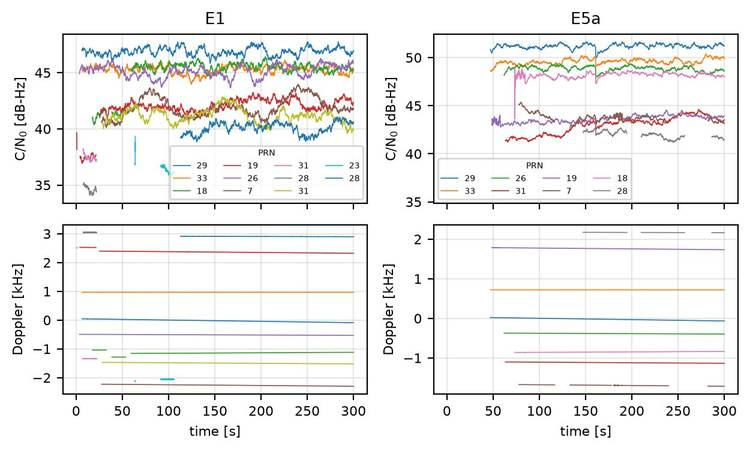
\includegraphics[width=1.0\linewidth]{gnss_sdr/x310_20261024T190000Z/galileo_tracking.jpg}
  \caption{Tracking: carrier-to-noise density ratio and carrier Doppler per satellite, while phase-locked (smooth Doppler curves = loops following the real satellite motion).}
\end{figure}

\begin{figure}[H]
  \centering
  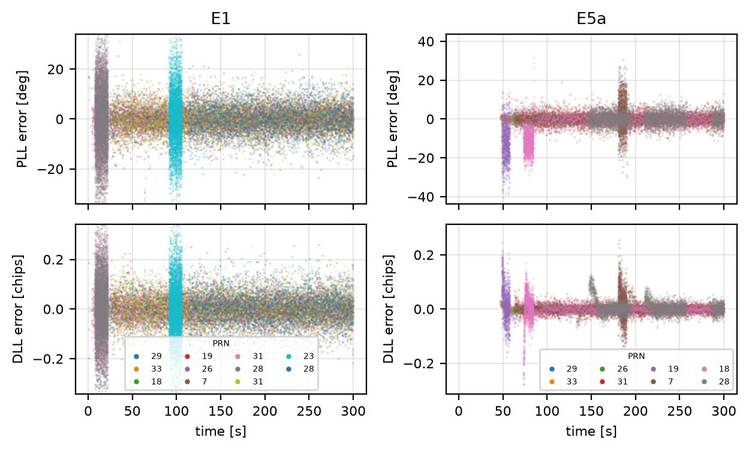
\includegraphics[width=1.0\linewidth]{gnss_sdr/x310_20261024T190000Z/galileo_tracking_errors.jpg}
  \caption{Tracking: loop errors per satellite while phase-locked, i.e. the discriminator outputs that the loops drive to zero: PLL carrier-phase error (degrees) and DLL code-delay error (chips) of every correlation. Noise centred on zero = clean tracking; its spread grows as C/N$_0$ drops, and jumps would mark cycle slips or a loop losing lock.}
\end{figure}

\begin{figure}[H]
  \centering
  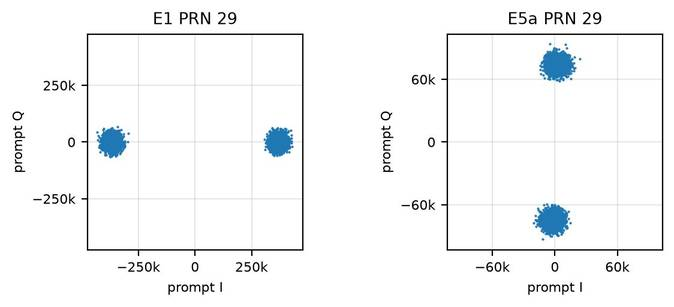
\includegraphics[width=1.0\linewidth]{gnss_sdr/x310_20261024T190000Z/galileo_tracking_iq.jpg}
  \caption{Tracking: prompt correlator outputs of the strongest satellite per band. Two tight clusters on one axis (the $\pm1$ data bits; GNSS-SDR's L5 tracking puts the data component on the Q axis), or, for the dataless pilots tracked for Galileo (E1-C, E5a-Q), the $\pm1$ chips of their secondary code, mean the PLL is phase-locked; a ring would mean it is not. \texttt{Prompt\_I}/\texttt{Prompt\_Q} are 32-bit floats (sums of the samples over one integration period, in file units): they never clip, only overflowing beyond $\pm 3.4\times10^{38}$, far above the $N\cdot\text{full scale}\cdot\sqrt{2}$ a sum of $N$ samples can reach.}
\end{figure}

\begin{table}[H]
  \centering
  \footnotesize
  \resizebox{\ifdim\width>\linewidth\linewidth\else\width\fi}{!}{%
  \begin{tabular}{lrrrrrrrr}
    \hline
    \textbf{Band} & \textbf{Ch.} & \textbf{PRN} & \textbf{Median C/N$_0$ [dB-Hz]} & \textbf{Phase-locked [\%]} & \textbf{Losses of lock} & \textbf{Tracked [s]} & \textbf{PLL error std [deg]} & \textbf{DLL error std [chips]} \\
    \hline
    E1 & 0 & 29 & 46.9 & 98 & 0 & 299 & 3.5 & 0.036 \\
    E1 & 1 & 33 & 45.3 & 98 & 0 & 299 & 3.7 & 0.038 \\
    E1 & 2 & 18 & 45.4 & 91 & 3 & 299 & 4.4 & 0.046 \\
    E1 & 3 & 19 & 42.0 & 98 & 1 & 299 & 6.3 & 0.065 \\
    E1 & 4 & 26 & 45.2 & 99 & 0 & 299 & 4.1 & 0.043 \\
    E1 & 5 & 7 & 41.8 & 98 & 1 & 277 & 5.7 & 0.061 \\
    E1 & 5 & 31 & 37.5 & 71 & 1 & 21 & 10.3 & 0.105 \\
    E1 & 6 & 28 & 34.9 & 68 & 1 & 21 & 14.2 & 0.139 \\
    E1 & 6 & 31 & 41.1 & 98 & 1 & 276 & 6.5 & 0.070 \\
    E1 & 7 & 23 & 39.8 & 14 & 5 & 105 & 12.1 & 0.116 \\
    E1 & 7 & 28 & 40.1 & 97 & 5 & 193 & 7.0 & 0.076 \\
    E5a & 8 & 29 & 51.2 & 52 & 0 & 274 & 1.3 & 0.007 \\
    E5a & 9 & 33 & 49.4 & 52 & 0 & 274 & 1.5 & 0.008 \\
    E5a & 10 & 26 & 48.4 & 31 & 1 & 274 & 1.7 & 0.008 \\
    E5a & 11 & 31 & 41.8 & 51 & 0 & 257 & 3.2 & 0.017 \\
    E5a & 12 & 19 & 43.4 & 91 & 0 & 254 & 9.0 & 0.050 \\
    E5a & 13 & 7 & 43.4 & 25 & 4 & 240 & 7.3 & 0.050 \\
    E5a & 14 & 18 & 48.2 & 100 & 0 & 227 & 7.4 & 0.044 \\
    E5a & 15 & 28 & 42.1 & 14 & 2 & 158 & 3.6 & 0.028 \\
    \hline
  \end{tabular}}
  \caption{Tracking: per channel and satellite (phase-locked: carrier lock test $> 0.8$; loop error standard deviations while phase-locked).}
\end{table}

\subsubsection{Telemetry decoder (Galileo E1 + E5a)}


\begin{figure}[H]
  \centering
  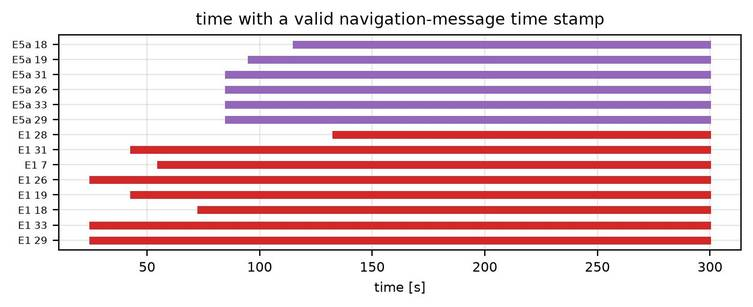
\includegraphics[width=1.0\linewidth]{gnss_sdr/x310_20261024T190000Z/galileo_telemetry.jpg}
  \caption{Telemetry decoder: per band and satellite, when the decoder delivered a valid transmit time (the first one comes after the first complete frame/message).}
\end{figure}

\begin{table}[H]
  \centering
  \footnotesize
  \resizebox{\ifdim\width>\linewidth\linewidth\else\width\fi}{!}{%
  \begin{tabular}{lrrrrr}
    \hline
    \textbf{Band} & \textbf{PRN} & \textbf{Messages decoded} & \textbf{Ephemeris} & \textbf{First valid at [s]} & \textbf{TOW [s]} \\
    \hline
    E1 & 7 & 24 & yes & 54.7 & 586880.0 \\
    E1 & 18 & 22 & yes & 72.7 & 586898.0 \\
    E1 & 19 & 24 & yes & 42.7 & 586868.0 \\
    E1 & 26 & 27 & yes & 24.7 & 586850.0 \\
    E1 & 28 & 16 & yes & 132.7 & 586958.0 \\
    E1 & 29 & 25 & yes & 24.7 & 586850.0 \\
    E1 & 31 & 25 & yes & 42.7 & 586868.0 \\
    E1 & 33 & 26 & yes & 24.7 & 586850.0 \\
    E5a & 18 & 10 & yes & 114.9 & 586940.3 \\
    E5a & 19 & 11 & yes & 94.9 & 586920.3 \\
    E5a & 26 & 12 & yes & 84.9 & 586910.3 \\
    E5a & 29 & 12 & yes & 84.9 & 586910.3 \\
    E5a & 31 & 12 & yes & 84.9 & 586910.3 \\
    E5a & 33 & 12 & yes & 84.9 & 586910.3 \\
    \hline
  \end{tabular}}
  \caption{Telemetry decoder: E1 I/NAV words, E5a F/NAV pages decoded, ephemeris obtained, and the first valid time of week.}
\end{table}

\subsubsection{Observables (Galileo E1 + E5a)}
Pseudorange, carrier phase and Doppler of every channel at common receiver epochs.

\begin{figure}[H]
  \centering
  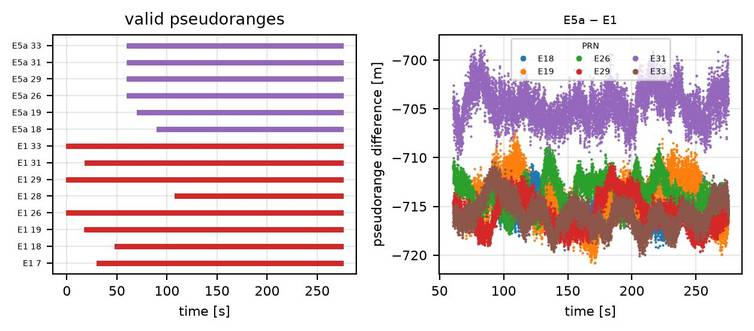
\includegraphics[width=1.0\linewidth]{gnss_sdr/x310_20261024T190000Z/galileo_observables.jpg}
  \caption{Observables: epochs with a valid pseudorange per band and satellite, and the difference between the two bands' pseudoranges of the same satellite (a constant receiver inter-band bias, the same for every satellite, plus the slowly varying ionospheric delay).}
\end{figure}

\begin{table}[H]
  \centering
  \footnotesize
  \resizebox{\ifdim\width>\linewidth\linewidth\else\width\fi}{!}{%
  \begin{tabular}{lrrrrrr}
    \hline
    \textbf{Difference} & \textbf{PRN} & \textbf{Common epochs} & \textbf{of run [\%]} & \textbf{Mean [m]} & \textbf{Std [m]} & \textbf{Drift [m/s]} \\
    \hline
    E5a $-$ E1 & 18 & 9240 & 62 & -715.18 & 1.29 & -0.0008 \\
    E5a $-$ E1 & 19 & 10241 & 68 & -714.24 & 2.20 & -0.0021 \\
    E5a $-$ E1 & 26 & 10728 & 72 & -713.77 & 1.56 & -0.0003 \\
    E5a $-$ E1 & 29 & 10727 & 72 & -715.68 & 1.65 & -0.0031 \\
    E5a $-$ E1 & 31 & 10726 & 72 & -704.59 & 1.77 & 0.0011 \\
    E5a $-$ E1 & 33 & 10727 & 72 & -715.80 & 1.51 & -0.0056 \\
    \hline
  \end{tabular}}
  \caption{Observables: pseudorange difference between the two bands of each satellite at common epochs (similar means = shared receiver bias; std = code noise of both bands).}
\end{table}

\subsubsection{PVT (Galileo E1 + E5a)}
Position from the pseudoranges and the decoded ephemeris, compared with the surveyed antenna position (-23.209433$^\circ$, -45.874875$^\circ$, 596.42~m).

\begin{figure}[H]
  \centering
  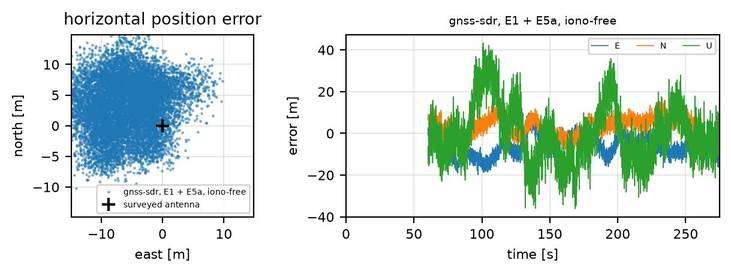
\includegraphics[width=1.0\linewidth]{gnss_sdr/x310_20261024T190000Z/galileo_pvt.jpg}
  \caption{PVT: position error with respect to the surveyed antenna position. gnss-sdr: GNSS-SDR's own RTKLIB solution.}
\end{figure}

\begin{table}[H]
  \centering
  \footnotesize
  \resizebox{\ifdim\width>\linewidth\linewidth\else\width\fi}{!}{%
  \begin{tabular}{l>{\centering\arraybackslash}p{4.2cm}}
    \hline
    \textbf{Solution} & \textbf{gnss-sdr, E1 + E5a, iono-free} \\
    \hline
    Solutions & 10909 \\
    Run with fix [\%] & 79 \\
    Mean E / N / U [m] & -6.0 / 3.2 / 0.0 \\
    Std E / N / U [m] & 4.8 / 4.5 / 13.5 \\
    RMS 2-D [m] & 9.4 \\
    RMS 3-D [m] & 16.4 \\
    95\% horiz. [m] & 15.1 \\
    \hline
  \end{tabular}}
  \caption{PVT: position error statistics with respect to the surveyed antenna (mean = accuracy, std = precision; \% of the run's seconds with a position; gnss-sdr outputs several solutions per second, gnss\_spp\_lib.py computes one per second).}
\end{table}

